%% =========================================================
%% Physical Review X (PRX) Template based on REVTeX 4-2
%% =========================================================

% options explain:
% aps: American Physical Society
% prx: Target journal Physical Review X
% reprint: Simulate final two-column publication look (use 'preprint' for submission if you prefer single column)
% superscriptaddress: Standard for multi-affiliations
% longbibliography: PRX requires full titles in references (Crucial!)
% nofootinbib: Footnotes go to bottom of page, not in bibliography

\documentclass[aps,prx,reprint,superscriptaddress,longbibliography,nofootinbib,floatfix]{revtex4-2}

%% Packages
\usepackage{graphicx}  % For figures
\usepackage{dcolumn}   % Align table columns on decimal point
\usepackage{bm}        % Bold math
\usepackage{amsmath}   % Math packages
\usepackage{amssymb}   % Math symbols
\usepackage{physics}   % Physics package (for \ket, \bra, \dd, etc. you used)
\usepackage{hyperref}  % Hyperlinks
\hypersetup{
    colorlinks=true,
    linkcolor=blue,
    citecolor=blue,
    urlcolor=blue
}
\usepackage{pifont}

\begin{document}

%% =========================================================
%% Title & Authors
%% =========================================================

\title{Transient Learning Dynamics Drive Escape from Sharp Valleys in Stochastic Gradient Descent}

%% Author 1
\author{Ning Yang}
\thanks{These authors contributed equally to this work.}
\affiliation{Peking University Chengdu Academy for Advanced Interdisciplinary Biotechnologies, Chengdu 610213, China}

%% Author 2
\author{Yikuan Zhang}
\thanks{These authors contributed equally to this work.}
\affiliation{School of Physics, Peking University, Beijing 100871, China}

%% Author 3
\author{Qi Ouyang}
\affiliation{Institute for Advanced Study in Physics, Zhejiang University, Hangzhou 310058, China}

%% Author 4
\author{Chao Tang}
\affiliation{Peking University Chengdu Academy for Advanced Interdisciplinary Biotechnologies, Chengdu 610213, China}
\affiliation{Center for Quantitative Biology, Peking University, Beijing 100871, China}

%% Author 5 (Corresponding)
\author{Yuhai Tu}
\email{ytu@flatironinstitute.org}
\affiliation{Center for Computational Biology \& Center for Computational Neuroscience, Flatiron Institute, New York, NY 10010, USA}

%% =========================================================
%% Abstract (Must be placed BEFORE \maketitle)
%% =========================================================
\begin{abstract}
Stochastic gradient descent (SGD) is central to deep learning, yet the dynamical origin of its preference for flatter, more generalizable solutions remains unclear. Here, by analyzing SGD learning dynamics, we identify a nonequilibrium mechanism governing solution selection. Numerical experiments reveal a transient exploratory phase in which SGD trajectories repeatedly escape sharp valleys and transition toward flatter regions of the loss landscape. By using a tractable physical model, we show that the SGD noise reshapes the landscape into an effective potential that favors flat solutions. Crucially, we uncover a transient freezing mechanism: as training proceeds, growing energy barriers suppress inter-valley transitions and ultimately trap the dynamics within a single basin. Increasing the SGD noise strength delays this freezing, which enhances convergence to flatter minima. Together, these results provide a unified physical framework linking learning dynamics, loss-landscape geometry, and generalization, and suggest principles for the design of more effective optimization algorithms.
\end{abstract}

\maketitle

%% =========================================================
%% Main Text
%% =========================================================

\section{Introduction}
Despite its substantial empirical success across numerous fields, the underlying mechanisms of deep learning remain poorly understood \cite{lecunDeepLearning2015,levineMachineLearningMeets2024a}. The training of a deep neural network can be viewed as the optimization of a high-dimensional loss landscape in parameter space \cite{liuLossLandscapesOptimization2022,sunGlobalLandscapeNeural2020,zhangEmbeddingPrincipleHierarchical2022}, formally expressed as
\begin{equation}
\mathcal{L}(\bm{\theta})=\frac{1}{M}\sum_{i=1}^M l(\bm{s}_i; \bm{\theta}),
\end{equation}
where $l(\bm{s}_i; \bm{\theta})$ denotes the loss associated with a single training sample $\bm{s}_i$ from a dataset of size $M$, and $\bm{\theta}$ represents the network’s parameter vector.

A prevailing hypothesis posits that the geometry of this loss landscape is intrinsically linked to the model's generalization ability \cite{choromanskaLossSurfacesMultilayer2015, huangUnderstandingGeneralizationVisualizations2020}. Specifically, solutions residing in ``flat'' or ``wide'' minima tend to generalize well to unseen data, whereas those in ``sharp'' or ``narrow'' minima are more prone to overfitting \cite{hochreiterFlatMinima1997,liVisualizingLossLandscape2018,jastrzebskiThreeFactorsInfluencing2018,wuHowSGDSelects2018,keskarLargeBatchTrainingDeep2017,chenSimpleConnectionLoss2024}. Recently, the relation between flatness of loss landscape at a solution with its generalization has been shown explicitly via an exact activity-weight duality \cite{fengActivityWeightDuality2023}. This flatness-generalization relation has led to the widespread view that the effectiveness of an optimizer is closely tied to its ability to locate flat minima.

Stochastic Gradient Descent (SGD) is the core optimizer of modern deep learning \cite{robbinsStochasticApproximationMethod1951,bottouLargeScaleMachineLearning2010}; despite its simplicity, it enables neural networks to achieve strong generalization. Unlike full-batch Gradient Descent (GD), which computes gradients over the entire dataset, SGD estimates the gradient using a randomly sampled mini-batch $\{\bm{s}_{\mu_i}\}_{i=1}^{B}$, ${\mu_i\in\{1,\cdots,M\}}$ of size $B$. The corresponding mini-batch loss is defined as
\begin{equation}
    \mathcal{L}^{\mu}(\bm{\theta})=\frac{1}{B}\sum_{i=1}^B l(\bm{s}_{\mu_i};\bm{\theta}),
\end{equation}
and the parameter update at iteration $t$ follows
\begin{equation} \label{eq:updating_rule_SGD}
    \bm{\theta}_{t+1}=\bm{\theta}_{t}-\eta \nabla_{\bm{\theta}} \mathcal{L}^{\mu}\left(\bm{\theta}_{t}\right), 
\end{equation}
where $\eta$ denotes the learning rate.

Due to mini-batch sampling, the noise covariance in SGD aligns with the Hessian matrix, making the noise both landscape-dependent and anisotropic \cite{xieOverlookedStructureStochastic2023,haochenShapeMattersUnderstanding2021}. 
This anisotropic stochasticity is believed to bias optimization trajectories toward flatter regions of the loss landscape \cite{fengInverseVarianceFlatness2021,zhuAnisotropicNoiseStochastic2019,xieDiffusionTheoryDeep2021,liHessianBasedAnalysis2020,yangStochasticGradientDescent2023}. 
Empirical studies further indicate that increasing the overall noise strength of SGD—by raising the learning rate $\eta$ or reducing the batch size $B$—typically leads to convergence toward flatter minima with improved generalization \cite{keskarLargeBatchTrainingDeep2017,chaudhariEntropySGDBiasingGradient2019,jastrzebskiThreeFactorsInfluencing2018}. In this view, gradient noise acts as an implicit regularizer, enabling the optimizer to escape sharp minima and explore broader regions of parameter space. However, most previous analyses studied this implicit regularization when the loss landscape can be approximated as a degenerate valley with negligible gradients \cite{zhuAnisotropicNoiseStochastic2019,xieDiffusionTheoryDeep2021,weiHowNoiseAffects2019,yangStochasticGradientDescent2023}. While this approximation holds in the late stages of training, the transient dynamics by which SGD selects flatter solutions during the early phase remain poorly understood.


Multiple studies have demonstrated the critical importance of the early phase of training, showing that key properties of the final network are established long before convergence \cite{gur-ariGradientDescentHappens2018,achilleCriticalLearningPeriods2019,fengPhasesLearningDynamics2021a,kalraPhaseDiagramEarly2023,jastrzebskiBreakEvenPointOptimization2020}. For instance, the ``lottery ticket hypothesis'' suggests that trainable subnetworks emerge very early in the training process \cite{frankleLotteryTicketHypothesis2019}. This raises a crucial question: How does SGD navigate the complex, high-dimensional loss landscape during these formative early stages to set the trajectory toward generalizable solutions? Understanding this ``early transient dynamic'' is essential for a complete theory of deep learning optimization.

In this paper, we systematically study how stochastic gradient descent (SGD) escapes sharp minima and preferentially converges toward flatter regions during early training when there are significant down-hill gradients. Combining empirical observations with a tractable theoretical model, we characterize the transient dynamics underlying this behavior. We identify a stochastic ``valley-jumping'' mechanism that enables SGD to explore multiple basins of attraction in the initial phase of optimization.

Our study provides a clear physical picture of transient learning dynamics. Anisotropic noise in SGD reshapes the loss landscape, giving rise to an emergent effective potential that systematically biases the dynamics toward flatter, more generalizable minima. Crucially, this exploratory behavior is intrinsically transient: as training proceeds, the evolving landscape geometry dynamically ``freezes'' the trajectory into a single valley. Higher noise levels—arising from larger learning rates or smaller batch sizes—prolong this pre-freezing regime, allowing the dynamics more time to follow the effective potential and discover flatter solutions. Taken together, these results offer a unified framework connecting stochasticity, loss landscape geometry, and generalization, and reveal an explicitly transient mechanism by which SGD preferentially selects flat minima.

\section{Results}
\subsection{SGD converges to distinct loss valleys separated by barriers}
To characterize the loss landscape explored by stochastic gradient descent (SGD), we first examine the endpoints of optimization. Starting from an identical initialization, we performed multiple training runs that differed only in random seed, batch size, and learning rate, using a 1,000-sample subset of the MNIST classification task and a fully connected neural network with two hidden layers (see Sec.~I~A in Supplemental Material for details).

The resulting training trajectories are shown in Fig.~\ref{fig:loss_landscape}\textit{A}, projected onto the first two principal components of the network parameters. Rather than converging to a single point, the trajectories cluster into several well-separated regions of parameter space, which we identify as distinct valleys of the loss landscape. All trajectories shown have fully converged and achieve 100\% training accuracy, indicating that each cluster corresponds to a local minimum separated from others by loss barriers.

Pairwise Jaccard similarity analysis, computed at the fully converged endpoints, further confirmed this clustered structure (Fig.~\ref{fig:loss_landscape}\textit{B}), defined as  
\begin{equation}
\mathrm{Sim}_J(\bm{\theta}^{(i)}, \bm{\theta}^{(j)}) \equiv
\frac{ \bigl|\mathcal{E}(\bm{\theta}^{(i)}) \cap \mathcal{E}(\bm{\theta}^{(j)})\bigr| }
     { \bigl|\mathcal{E}(\bm{\theta}^{(i)}) \cup \mathcal{E}(\bm{\theta}^{(j)})\bigr| },
\end{equation}  
where $\mathcal{E}(\bm{\theta}^{(i)})$ denotes the set of misclassified test samples for solution $\bm{\theta}^{(i)}$. Unlike similarity measures defined directly in weight space, which suffer from permutation symmetry of neurons, this error-based similarity is invariant to such symmetries and thus provides a more faithful measure of solution similarity. Finally, Hessian spectra computed at these endpoints provide additional evidence for the valley structure: a few near-zero eigenvalues correspond to flat directions along the valley floor, while many large eigenvalues indicate steep walls (see Sec.~I~B in Supplemental Material and Fig.~S1), consistent with previous studies \cite{wuHowSGDSelects2018,ghorbaniInvestigationNeuralNet2019,chaudhariEntropySGDBiasingGradient2019}.

These valleys are not smoothly connected but are separated by substantial loss barriers. Linear interpolation between two final solutions, $\bm{\theta}^{(i)}$ and $\bm{\theta}^{(j)}$, demonstrates this separation. To quantify this effect, we define the loss barrier $\Delta \mathcal{L}_\mathrm{barrier}$ as
\begin{equation}
\begin{split}
\Delta \mathcal{L}_\mathrm{barrier}(\bm{\theta}^{(i)}, \bm{\theta}^{(j)}) 
&\equiv \max_{\alpha \in [0,1]} 
   \mathcal{L}\!\left(\alpha \bm{\theta}^{(i)} + (1-\alpha)\bm{\theta}^{(j)}\right)  \\[6pt]
&\quad - \frac{\mathcal{L}(\bm{\theta}^{(i)}) + \mathcal{L}(\bm{\theta}^{(j)})}{2},
\end{split}
\end{equation}
where $\alpha$ is the interpolation coefficient. For highly similar solutions ($Sim_J=0.95$), the interpolation path exhibits a negligible barrier (Fig.~\ref{fig:loss_landscape}\textit{C}). In contrast, dissimilar solutions ($Sim_J=0.625$) are separated by a pronounced barrier that must be crossed to move from one valley to another (Fig.~\ref{fig:loss_landscape}\textit{D}). Tracking these interpolation paths over training time further shows that such barriers emerge early in the optimization process. 

Moreover, this trend is robust: plotting barrier height against solution similarity across many pairs reveals a clear negative correlation, indicating that more dissimilar solutions are separated by higher loss barriers (Fig.~\ref{fig:loss_landscape}\textit{E}; linear fit $R^2=0.64$).  Together, these results depict the neural network loss landscape as a complex terrain of multiple valleys, separated by barriers whose heights reflect the functional dissimilarity of the solutions they contain.

% Figure 1
\begin{figure*}[t]
\centering
\includegraphics[width=0.9\textwidth]{Figures/Fig1_solution_valleys.pdf}
\caption{The loss landscape of a neural network is composed of multiple distinct solution valleys separated by loss barriers.
(\textit{A}) A 2D Principal Component Analysis (PCA) projection of the weight training trajectories on subset of MNIST. All runs start from an identical initialization (star) but use different SGD hyperparameters (learning rate $\eta$ and batch size $B$), indicated by different colors and marker styles, respectively. The trajectories shown here all converge, achieving 100\% training accuracy.
(\textit{B}) The Jaccard similarity ($\mathrm{Sim}_J$) matrix between pairs of solutions, calculated based on the overlap of misclassified test samples.
(\textit{C, D}) The training loss along the linear interpolation path between two final solutions. A negligible loss barrier exists for highly similar solutions ($\mathrm{Sim}_J = 0.95$) (\textit{C}), while a significant barrier separates dissimilar solutions ($\mathrm{Sim}_J = 0.625$) (\textit{D}). The color scale represents the normalized training time $t/t_\mathrm{max}$.
(\textit{E}) The height of the loss barrier $\Delta \mathcal{L}_\mathrm{barrier}$ exhibits a strong negative correlation with the Jaccard similarity $\mathrm{Sim}_J$ between solution pairs (linear fit, $R^2=0.64$).}
\label{fig:loss_landscape}
\end{figure*}

\subsection{Increased SGD noise promotes convergence to flatter, more generalizable valleys}

Stochasticity in SGD arises primarily from mini-batch sampling, with its magnitude controlled by the batch size $B$ and learning rate $\eta$: smaller $B$ or larger $\eta$ produces stronger noise \cite{jastrzebskiThreeFactorsInfluencing2018}. To systematically access its effects, we trained networks over a broad range of $(\eta, B)$ combinations, spanning learning rates from $\eta = 0.001$ to $0.1$ and batch sizes from $B = 10$ to $1{,}000$, where the latter corresponds to full-batch gradient descent. For each parameter setting, we performed 20 independent training runs starting from identical initial conditions (see Sec.~I~A in Supplemental Material).

As expected, increased SGD noise led to more diverse final solutions. This diversity is captured quantitatively by the average pairwise Jaccard similarity $\langle Sim_J \rangle$ between independent realizations for each hyperparameter setting (Fig.~\ref{fig:solution_properties}\textit{A}). Low-noise settings (large $B$, small $\eta$) produced solutions that were highly similar, whereas higher noise (smaller $B$ or larger $\eta$) systematically reduced $\langle Sim_J \rangle$, indicating broader exploration of the loss landscape. This trend is further visualized in PCA-projected weight space: the training trajectories for a low-noise example ($B=50, \eta=0.01$, \ding{172} in Fig.~\ref{fig:solution_properties}\textit{A}) cluster tightly (Fig.~\ref{fig:solution_properties}\textit{B}), whereas the high-noise example ($B=50, \eta=0.05$, \ding{173} in Fig.~\ref{fig:solution_properties}\textit{A}) spreads over a wider region of PCA space (Fig.~\ref{fig:solution_properties}\textit{C}), highlighting the role of noise in enabling broader exploration.

Crucially, this exploration is biased toward more generalizable solutions: higher noise systematically yielded solutions with higher maximum test accuracy $\max(Acc_\mathrm{test})$ (Fig.~\ref{fig:solution_properties}\textit{D}). These higher-performing solutions also lie in flatter valleys: here, we quantified flatness $F$ as the inverse geometric mean of the top $N$ non-degenerate Hessian eigenvalues,
\begin{equation}
F \equiv \left( \prod_{i=1}^{N} \lambda_i(\mathbf{H}) \right)^{-\tfrac{1}{N}},
\end{equation}
where we set $N=10$ for the 10-class MNIST task \cite{sagunEmpiricalAnalysisHessian2018a}. Increasing noise consistently steered optimization toward flatter minima (Fig.~\ref{fig:solution_properties}\textit{F}). Direct comparisons further confirmed that smaller $B$ yields solutions that are both flatter and more accurate (Fig.~\ref{fig:solution_properties}\textit{E}\&\textit{G}), reinforcing the well-established link between flatness and generalization \cite{hochreiterFlatMinima1997,liVisualizingLossLandscape2018,jastrzebskiThreeFactorsInfluencing2018,wuHowSGDSelects2018,keskarLargeBatchTrainingDeep2017,chenSimpleConnectionLoss2024}. 


Overall, these results indicate that SGD noise functions not merely as an implicit regularizer but as an active exploration mechanism: by promoting broader exploration of the parameter space, higher noise systematically guides optimization toward flatter valleys associated with improved generalization.

% Figure 2
\begin{figure*}[t]
\centering
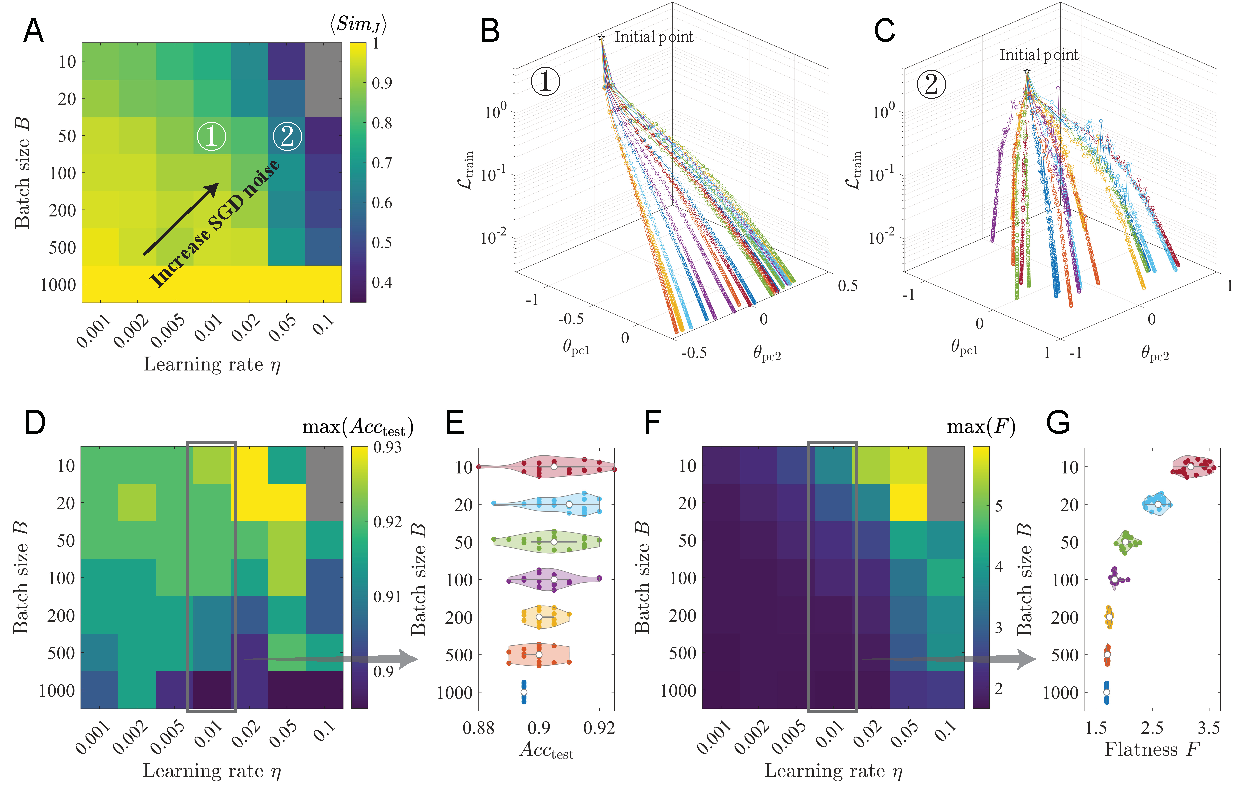
\includegraphics[width=0.9\textwidth]{Figures/Fig2_solution_properties_different_noise.pdf}
\caption{Increased SGD noise promotes broader exploration and convergence to flatter, more generalizable valleys. 
(\textit{A}) Heatmap of average Jaccard similarity $\langle \mathrm{Sim}_J \rangle$ between final solutions across learning rates $\eta$ and batch sizes $B$ ($B=1000$ corresponds to full-batch Gradient Descent). 
(\textit{B, C}) PCA-projected training trajectories for low-noise ($B=50, \eta=0.01$, \ding{172} in \textit{A}) and high-noise ($B=50, \eta=0.05$, \ding{173} in \textit{A}) conditions. 
(\textit{D, F}) Heatmaps of maximum test accuracy $\max(Acc_{\mathrm{test}})$ (\textit{D}) and maximum solution flatness $\max(F)$ (\textit{F}), where flatness is quantified as the inverse geometric mean of the top Hessian eigenvalues. 
(\textit{E, G}) Violin plots showing the distributions of test accuracy (\textit{E}, for $\eta=0.05$, gray box in \textit{D}) and flatness (\textit{G}) across batch sizes. Gray regions in the heatmaps (\textit{A, D, F}) indicate divergent settings where no runs achieve 100\% training accuracy and are therefore excluded from comparisons with other conditions. See Sec.~I~A in Supplemental Material for details and Fig.~S2 for additional numerical results. 
}
\label{fig:solution_properties}
\end{figure*}

\subsection{Larger SGD noise extends the transient search phase of training}

Having established that SGD noise biases optimization toward flatter, more generalizable valleys, we next examine the learning dynamics underlying this effect. Training typically begins with a rapid decrease in the loss, corresponding to a transient search phase during which the optimizer explores multiple regions of the loss landscape. We define the end of this phase as the freezing time, $t_{\mathrm{freeze}}$, given by the first iteration at which the training loss drops below a small threshold $\mathcal{L}_c$:
\begin{equation}
t_{\mathrm{freeze}} \equiv \min \{\, t \mid \mathcal{L}_{\mathrm{train}}(t) < \mathcal{L}_c \,\}.
\end{equation}
In our experiments, we set $\mathcal{L}_c = 0.1$; varying this threshold does not affect the qualitative conclusions (see Sec.~I~D in Supplemental Material and Fig.~S3). Beyond $t_{\mathrm{freeze}}$, training accuracy approaches 100\%, and the dynamics become confined to the basin of attraction of a single valley (Fig.~\ref{fig:early_dynamics}\textit{A}).


We then investigated how SGD noise influences the duration of this transient exploration phase. While different noise levels (controlled via batch size $B$) lead to comparable final training losses, higher noise systematically delays entry into the low-loss regime. In particular, reducing $B$ increases $t_{\mathrm{freeze}}$ (Fig.~\ref{fig:early_dynamics}\textit{B}), indicating that optimizers with larger noise spend more time exploring the landscape before settling into a valley. A phase map of the normalized freezing time, $\eta \langle t_{\mathrm{freeze}} \rangle$ (where $\eta$ sets the iteration time interval), across a wide hyperparameter range further confirms this trend: the duration of the early transient phase consistently grows with increased SGD noise (Fig.~\ref{fig:early_dynamics}\textit{C}).

Importantly, this extended exploration period is not wasted. It is precisely during this phase that the optimizer discovers flatter regions of the landscape. Tracking the evolution of flatness during training shows a continuous increase (except at the very beginning, where gradients are extremely large) across all noise levels (Fig.~\ref{fig:early_dynamics}\textit{D}). Notably, high-noise trajectories (small $B$) not only prolong the exploration period but also leverage it to locate progressively flatter regions, ultimately converging to solutions with substantially greater flatness than their low-noise counterparts. 

These results establish a direct link between the duration of the noise-driven transient phase and the geometric quality of the final solution: the longer the optimizer explores before freezing, the flatter the valley it is likely to reach.

\begin{figure}[tbhp]
\centering
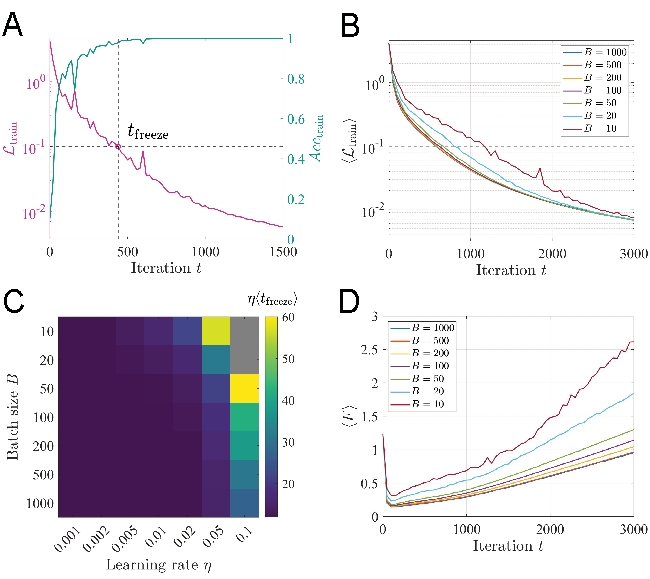
\includegraphics[width=\linewidth]{Figures/Fig3_early_stage_dynamics.pdf}
\caption{SGD noise extends the transient phase and facilitates the discovery of flatter solutions. 
(\textit{A}) Representative training trajectory showing training loss (magenta) and accuracy (cyan) for $B=50$ and $\eta=0.05$. The freezing time $t_{\mathrm{freeze}}$ is defined as the first iteration where the training loss drops below $\mathcal{L}_c=0.1$. 
(\textit{B}, \textit{D}) Mean training loss $\langle \mathcal{L}_{\mathrm{train}} \rangle$ (\textit{B}) and mean flatness $\langle F \rangle$ (\textit{D}) across multiple runs for different batch sizes $B$ at fixed learning rate $\eta=0.02$. 
(\textit{C}) Heatmap of normalized mean freezing time $\eta \langle t_{\mathrm{freeze}} \rangle$ across learning rates and batch sizes, averaged over all runs that reached $\mathcal{L}_c$. Gray regions in heatmaps indicate settings where no runs reach 100\% training accuracy.} 
\label{fig:early_dynamics}
\end{figure}

\subsection{Continuation training experiments reveal valley escapes during early transient phase}

To directly visualize how SGD transitions between valleys, we designed a {\it continuation training} experiment. A network was first trained using SGD to generate a reference trajectory (Fig.~\ref{fig:continue_training}\textit{A}; reference setting $B = 50$, $\eta = 0.05$). At selected times $t_c$ along this trajectory, training was branched and resumed using full-batch gradient descent (GD) with the same learning rate. Because GD is deterministic, it rapidly descends into the local valley specified by its initialization, without further stochastic exploration. The final solutions obtained from these continuations therefore identify the valley occupied by the SGD trajectory at time $t_c$ (Fig.~\ref{fig:continue_training}\textit{A}; see Sec.~I~E in Supplemental Material for details). This procedure enables a direct reconstruction of the sequence of valleys explored by SGD during the early stages of training.

The results provide direct evidence for valley jumping during the early stages of training. Continuations from very early times (e.g., $t_c=20$) converge to solutions characterized by high test loss and low flatness (Fig.~\ref{fig:continue_training}\textit{B}, \textit{C}). As $t_c$ increases, however, the trajectories branched at later times progressively converge to better solutions, landing in valleys with both lower test loss and higher flatness (inset of Fig.~\ref{fig:continue_training}\textit{B}, \textit{C}). This indicates that the SGD trajectory does not remain trapped in its initial basin of attraction, but instead transitions across the landscape to discover flatter and more generalizable regions. The improvement is systematic: the final test loss and flatness of these solutions are strongly correlated ($R^2=0.76$), confirming that the search for flatter valleys is effectively the search for better generalization (Fig.~\ref{fig:continue_training}\textit{D}).

We further found that valley jumping occurs almost exclusively before the freezing time $t_{\mathrm{freeze}}$. To quantify this effect, we computed the Jaccard similarity $Sim_J$ between final solutions obtained from different continuation times. Similarities remain low between solutions at early continuation times but increase steadily, approaching 1 as $t_c$ nears $t_{\mathrm{freeze}}$ (Fig.~\ref{fig:continue_training}\textit{E}). This pattern indicates that substantial transitions between distinct valleys occur almost entirely during the transient phase of training. Once this phase is surpassed ($t_c \geq t_{\mathrm{freeze}}$, red square region in Fig.~\ref{fig:continue_training}\textit{E}), the SGD trajectory stabilizes and remains confined to a single, high-quality valley.

Together, these results from the continuation training experiments indicate that SGD drives valley transitions during the transient phase, guiding the trajectory to escape from sharper minima and progressively converge into flatter, more generalizable ones.

\begin{figure*}[tbhp]
\centering
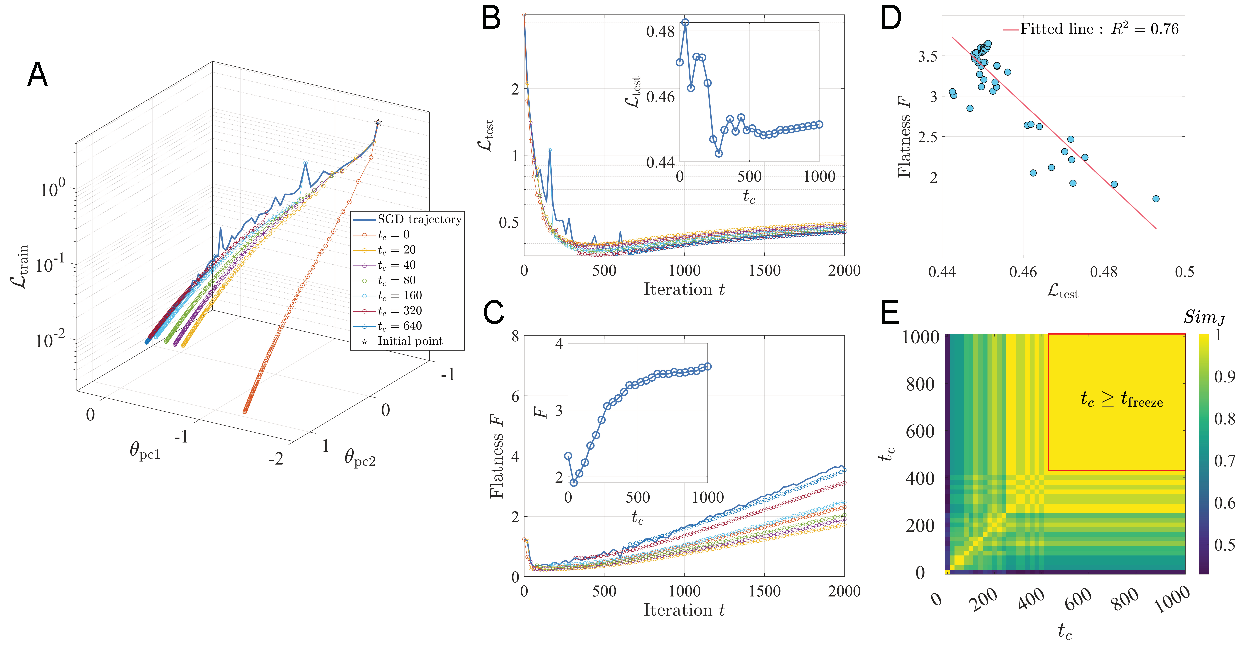
\includegraphics[width=0.9\textwidth]{Figures/Fig4_escaping_behavior.pdf}
\caption{Continuation training reveals the valley-jumping dynamics of SGD during the early transient phase.
(\textit{A}) A 2D PCA projection of the main SGD trajectory (blue solid line; reference setting $B=50$, $\eta=0.05$) and trajectories obtained by switching to full-batch GD ($B=1000$, $\eta=0.05$) at different branching times $t_c$ (colored lines with circle markers).
(\textit{B, C}) Evolution of the test loss $\mathcal{L}_\mathrm{test}$ (\textit{B}) and solution flatness $F$ (\textit{C}) for the main SGD trajectory and the GD-continued trajectories branched at different $t_c$. Insets show the final values of $\mathcal{L}_{\mathrm{test}}$ and $F$ for each continuation trajectory (evaluated at $t=2000$) as a function of their branching time $t_c$.
(\textit{D}) Final flatness $F$ of the continued solutions exhibits a strong negative correlation with their final test loss $\mathcal{L}_\mathrm{test}$ (linear fit, $R^2=0.76$).
(\textit{E}) Jaccard similarity $Sim_J$ among solutions obtained from different branching times $t_c$, with the red square marking the region where $t_c \geq t_{\mathrm{freeze}}$.}
\label{fig:continue_training}
\end{figure*}

\subsection{A minimal two-valley model recapitulates empirical training dynamics}
As described above, in real training we empirically observe the following features: (1) the loss landscape splits into multiple solution valleys originating from a common starting point, each characterized by a different degree of flatness; (2) as training proceeds and the loss decreases, the valleys become increasingly flatter, reflecting a systematic growth of flatness; (3) due to stochastic mini-batch sampling, the SGD trajectory may transiently jump from shaper valleys during the early phase of optimization; and (4) increasing the level of SGD noise systematically delays the valley-jumping freezing time, thereby biasing the dynamics toward convergence into the flatter valley. This physical picture is schematically illustrated in Fig.~\ref{fig:toy_model}\textit{A}, which bears a strong resemblance to the Waddington epigenetic landscape where cells traverse a bifurcating potential surface to achieve stable developmental fates \cite{waddington1957strategy, kitanoTheoryBiologicalRobustness2007, wangQuantifyingWaddingtonLandscape2011, pujadasRegulatedNoiseEpigenetic2012,ferrellBistabilityBifurcationsWaddingtons2012}.

To explain these phenomena within a minimal yet analytically tractable framework, we construct a two-dimensional loss landscape $\mathcal{L}(x, y)$ that takes the form of a bifurcating valley (Fig.~\ref{fig:toy_model}\textit{B}). Here, the variable $y$ represents the principal training direction along which the overall loss decreases, whereas $x$ denotes a symmetry-breaking parameter direction where the valley bifurcation emerges. The loss is defined piecewise as
\begin{equation}
    \mathcal{L}(x, y) = \mathcal{L}_0(y)  +
    \begin{cases}
       \dfrac{x(x - g_1(y))}{f_1(y)}, & x \geq 0, \\
       \dfrac{x(x + g_2(y))}{f_2(y)}, & x < 0,
    \end{cases}
    \label{eq:loss_toy_model}
\end{equation}
with several components controlling the landscape geometry. The functions $g_{1,2}(y)$ set the valley positions:
\begin{equation}
    g_1(y) = \frac{2 x_1 y}{y + y_b}, \qquad 
    g_2(y) = \frac{2 x_2 y}{y + y_b},
\end{equation}
so that the valley minima $x_{1,2}^{\star}$ are located at $x_1^{\star} = g_1(y)/2$ and $x_2^{\star} = -g_2(y)/2$, asymptotically approaching $x_1$ and $-x_2$ as $y \to \infty$. The parameter $y_b$ sets the bifurcation scale, controlling how rapidly the valleys separate. The valley flatness (inverse curvatures) are determined by $f_{1,2}(y)$:
\begin{equation}
    f_1(y) = f_0 \frac{x_1^2}{x_0^2} \frac{(y+y_f)^2}{(y+y_b)^2}, 
    \qquad 
    f_2(y) = f_0 \frac{x_2^2}{x_0^2} \frac{(y+y_f)^2}{(y+y_b)^2},
\end{equation}
where $f_0$ sets the overall flatness scale, $x_0$ is a normalization constant, and $y_f$ controls the rate at which both valleys flatten as $y$ increases. Note that while the absolute flatness evolves, their ratio remains constant. We define this flatness ratio as $\gamma \equiv f_1(y)/f_2(y) = (x_1/x_2)^2$. Since $x_1 > x_2$, we have $\gamma > 1$, indicating that the valley with $x>0$ is flatter.

For simplicity, the landscape is constructed to disentangle the geometric effect of flatness from valley depth. The two minima, located at $x^{\star}_1(y)$ and $x^{\star}_2(y)$, are designed to have equal depths relative to the barrier at $x=0$. This common depth defines the barrier height $\Delta \mathcal{L}(y)$, which evolves with $y$ according to
\begin{equation}
\begin{split}
    \Delta \mathcal{L}(y) 
    &= \mathcal{L}(0, y) - \mathcal{L}(x_1^{\star}, y) 
     = \mathcal{L}(0, y) - \mathcal{L}(x_2^{\star}, y)  \\
    &= \frac{x_0^2}{f_0} \frac{y^2}{(y+y_f)^2}.
\end{split}
\end{equation}
The barrier height increases with $y$ and saturates at $x_0^2/f_0$ as $y \to \infty$. Furthermore, we introduce a global drift term
\begin{equation}
    \mathcal{L}_0(y) = \mathcal{L}_d e^{-y / y_d} + \mathcal{L}_0^{\star},
\end{equation}
which adds a weak, decaying bias along the $y$-direction and captures the overall loss reduction typically induced by the cross-entropy function during training. Here, $\mathcal{L}_d$ controls the initial bias strength and $y_d$ sets its decay scale along $y$. A constant offset $\mathcal{L}_0^{\star} = x_0^2 / f_0$ is included to ensure that $\mathcal{L} \ge 0$ across the entire landscape.

The learning dynamics are described by a discrete-time Langevin equation. At each iteration, the position $\bm{\theta}=(x,y)$ evolves as
\begin{equation}
    \bm{\theta}_{t+1} = \bm{\theta}_t - \eta \bigl( \nabla \mathcal{L}(\bm{\theta}_t) + \bm{\xi}_t \bigr),
\label{eq:SGD_updating_rule}
\end{equation}
where $\eta$ is the learning rate. The noise term $\bm{\xi}_t$ is sampled from a zero-mean Gaussian distribution
\begin{equation}
    \bm{\xi}_t \sim \mathcal{N}\bigl(0, \mathbf{\Sigma}(\bm{\theta}_t)\bigr).
\end{equation}
In SGD, this gradient noise is empirically observed to be highly anisotropic and strongly correlated with the local geometry of the loss landscape~\cite{fengInverseVarianceFlatness2021,zhuAnisotropicNoiseStochastic2019,xieDiffusionTheoryDeep2021,liHessianBasedAnalysis2020,yangStochasticGradientDescent2023}. To capture this landscape-dependent noise, we model the noise covariance as proportional to the local Hessian $\mathbf{H}(\bm{\theta}_t)$:
\begin{equation}
    \mathbf{\Sigma}(\bm{\theta}_t) = 2\sigma \mathbf{H}(\bm{\theta}_t),
\end{equation}
where $\sigma$ sets the noise strength, inversely dependent on batch size $B$. Note that the qualitative behavior of our model is insensitive to the exact functional dependence between $\mathbf{\Sigma}$ and $\mathbf{H}$. Any monotonically increasing relationship (e.g., $\mathbf{\Sigma}\propto \mathbf{H}$ or $\mathbf{\Sigma}\propto \mathbf{H}^2$) yields the same behavior (see Sec.~II~B in Supplemental Material and Fig.~S6 for details).


Simulations of this model reproduce our key empirical findings. Starting from the two valleys with equal probabilities, we varied $\eta$ and $\sigma$ and measured the probability of converging to the flatter valley $P_{\mathrm{flat}}$ and the normalized mean freezing time $\eta \langle t_{\mathrm{freeze}} \rangle$, defined as the last valley-switching iteration (see Sec.~II~A in Supplemental Material for details). The results reveal a sharp transition: larger $\eta$ or $\sigma$ dramatically increase the likelihood of convergence to the flatter valley (Fig.~\ref{fig:toy_model}\textit{C}), consistent with our empirical observation that stronger SGD noise biases solutions toward flatter minima (compare with Fig.~\ref{fig:solution_properties}\textit{F}). Moreover, the model reproduces the link between noise and transient exploration. The normalized freezing time increases systematically with both $\eta$ and $\sigma$ (Fig.~\ref{fig:toy_model}\textit{D}). This parallels our neural network experiments (compare with Fig.~\ref{fig:early_dynamics}\textit{C}). 

Despite its simplicity, the two-valley model captures the essential features of the learning dynamics: the anisotropic landscape-dependent noise not only enables escape from sharper minima but also biases convergence toward flatter regions by extending the early transient exploration phase, thereby allowing the dynamics to settle preferentially into flatter solution valleys. Next, we analytically elucidate the underlying mechanisms for valley selection during the early exploratory learning phase in the two-valley model. 

\begin{figure}[tbhp]
\centering
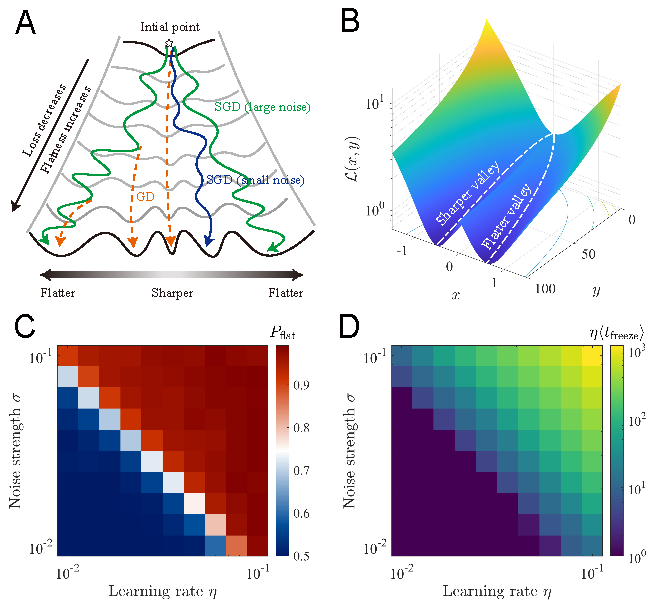
\includegraphics[width=\linewidth]{Figures/Fig5_toy_model.pdf}
\caption{A minimal two-valley model with anisotropic, landscape-dependent noise recapitulates the empirically observed training dynamics. 
(\textit{A}) Conceptual schematic of key characteristics of empirical SGD dynamics. 
(\textit{B}) The constructed 2D loss landscape $\mathcal{L}(x, y)$ with bifurcating sharper and flatter valleys of equal depth, as defined in Eq.~\ref{eq:loss_toy_model}. 
(\textit{C} and \textit{D}) Heatmaps showing the probability of converging to the flatter valley $P_{\mathrm{flat}}$ (\textit{C}) and the normalized mean freezing time $\eta \langle t_{\mathrm{freeze}} \rangle$ (\textit{D}), as functions of learning rate $\eta$ and noise strength $\sigma$. Statistics were collected from 2000 simulations, half initialized on the sharper side and half on the flatter side for each hyperparameter setting. Full simulation procedures and landscape parameters are provided in the Supplemental Material, Sec.~II~A.
}
\label{fig:toy_model}
\end{figure}


\subsection{SGD favors flatter minima in the quasi–steady-state regime}

In the limit of small learning rates, the discrete SGD updates in Eq.~\ref{eq:SGD_updating_rule} can be approximated by a continuous-time stochastic process. In this regime, the learning dynamics are governed by a continuous-time Langevin equation, and the probability density $P(x,y,t)$ for the system to occupy position $(x,y)$ at time $t$ evolves according to a corresponding Fokker--Planck equation:
\begin{equation}
\partial_t P
= \nabla \cdot \left[ P \nabla \mathcal{L} + \mathbf{D} \cdot \nabla P\right].
\end{equation}

The landscape-dependent noise leads to an anisotropic diffusion tensor $\mathbf{D}(x,y)$, expressed as
\begin{equation}
\mathbf{D}(x,y) = \tfrac{1}{2}\eta\mathbf{\Sigma}(x,y) = \Delta_S \mathbf{H}(x,y),
\end{equation}
where the effective noise level of SGD is defined as the product of the learning rate and noise strength, i.e., $\Delta_S \equiv \eta\sigma$ (see Appendix~\ref{sec:appendix1} for details).    

The dynamics involve several characteristic timescales: the local relaxation time in the $x$-direction, $\tau_x \sim f_{1(2)}(y)$, and the longitudinal drift time in the $y$-direction, $\tau_y \sim |\mathrm{d}y/\mathrm{d}t|^{-1}$. When $\tau_x \ll \tau_y$, the fast variable $x$ rapidly relaxes to a local equilibrium at an approximately fixed $y$, which evolves at a much longer timescale. In this quasi-steady-state regime, the conditional probability distribution $P_\mathrm{ss}^{\pm}(x|y)$ takes the form:
\begin{equation}
    P_\mathrm{ss}^{\pm}(x|y) \approx 
    \frac{1}{Z_\mathrm{ss}^{\pm}(y)}
    \exp\!\left(\frac{\mathcal{L}_0(y) - \mathcal{L}(x,y)}{D_{11}^{\pm}(y)}\right),
\end{equation}
where $D_{11}^{\pm}(y) = 2\Delta_S / f_{1(2)}(y)$ are the diffusion coefficients in the two valleys, and $Z_\mathrm{ss}^{\pm}(y)$ are the corresponding normalization constants. Here and throughout, the superscripts “$+$” and “$-$” denote quantities associated with the flatter and sharper valleys, respectively. 

The landscape-dependent, anisotropic noise inherent to SGD violates the fluctuation–dissipation theorem, highlighting the intrinsically nonequilibrium nature of the learning dynamics. In the quasi–steady-state regime $(\tau_x\ll \tau_y)$, the joint steady-state distribution can be approximated as $P_{\mathrm{ss}}(x,y) \approx P_{\mathrm{ss}}(x|y)P_{\mathrm{ss}}(y)$. Solving for $P_{\mathrm{ss}}(x,y)$ reveals that the learning dynamics effectively explores a noise-induced nonequilibrium loss landscape, described by an effective potential $\mathcal{L}_{\mathrm{eff}}(x,y)$ that explicitly depends on the SGD noise strength:
\begin{equation}
\begin{split}
    \mathcal{L}_{\mathrm{eff}}^{\pm}(x,y)
    &\equiv -T_{\mathrm{eff}}(y)\ln P_\mathrm{ss}^{\pm}(x,y)  \\
    &\approx 
    \gamma^{\pm\frac{1}{2}}\mathcal{L}(x,y)
    +\left(1-\gamma^{\pm\frac{1}{2}}\right)\mathcal{L}_0(y),
\end{split}
\label{eq:effective_loss_SGD}
\end{equation}
where $T_{\mathrm{eff}}(y) \equiv \sqrt{D_{11}^{+}(y)D_{11}^{-}(y)} = 2\Delta_S / \sqrt{f_1(y)f_2(y)}$ denotes the effective temperature.  

This effective loss can be decomposed into the original loss $\mathcal{L}(x,y)$ and an additional correction term $\mathcal{L}_{\mathrm{SGD}}(x,y)$ that arises solely from the anisotropic nature of the SGD noise (see Appendix~\ref{sec:appendix2} for detailed derivation):
\begin{equation}
\begin{split}
    \mathcal{L}_{\mathrm{SGD}}^{\pm}(x,y)
    &\equiv \mathcal{L}_{\mathrm{eff}}^{\pm}(x,y)-\mathcal{L}(x,y) \\
    &= \left(\gamma^{\pm\frac{1}{2}}-1\right)
    \big[\mathcal{L}(x,y)-\mathcal{L}_0(y)\big].
\end{split}
\end{equation}
Since the flatness ratio satisfies $\gamma > 1$, the SGD correction term lowers the effective loss near the flat minimum while raising it near the sharp one, as shown in Fig.~\ref{fig:analytical_results}\textit{A}. 

\begin{figure*}[t]
\centering
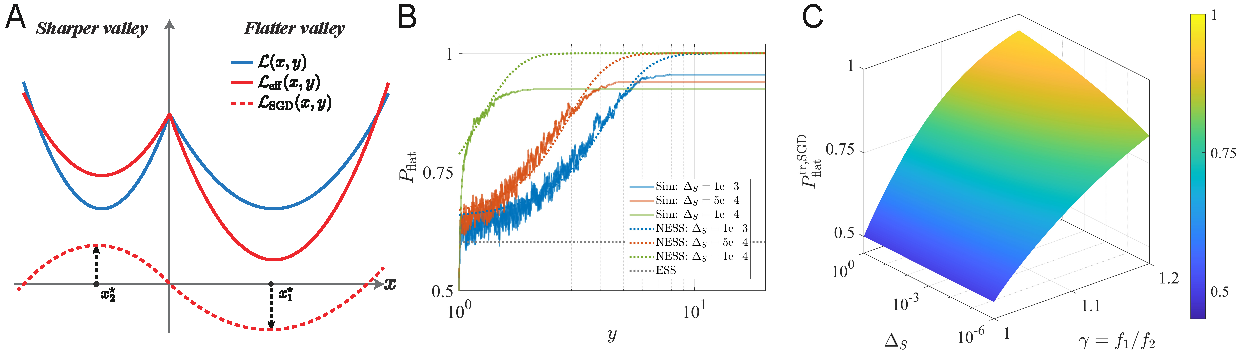
\includegraphics[width=0.9\textwidth]{Figures/Fig6_analytical_model.pdf}
\caption{Analytical theory reveals that a transient "freezing" mechanism explains the preference for flatter valleys.
(\textit{A}) Anisotropic SGD noise reshapes the original loss $\mathcal{L}(x,y)$ (blue solid line) into an effective loss $\mathcal{L}_{\mathrm{eff}}(x,y)$ (red solid line) where adding a correction term $\mathcal{L}_{\mathrm{SGD}}(x,y)$ (red dashed line). 
(\textit{B}) Comparison of the simulated flat-valley probability $P_{\mathrm{flat}}$ (solid lines) with theoretical nonequilibrium steady-state (NESS) predictions (dotted lines, Eq.~\ref{eq:ss_SGD}) for different noise levels $\Delta_S$. The equilibrium steady-state (ESS) probability $P_{\mathrm{flat}}^{\mathrm{eq}}= (1+\gamma^{-1})^{-1}$ is marked by black dotted line.
(\textit{C}) The final flat-valley probability predicted by the transient theory ($P_{\mathrm{flat}}^{\mathrm{tr,SGD}}$, Eq.~\ref{eq:tr_SGD}) with effective noise strength $\Delta_S$ and flatness ratio $\gamma=f_1/f_2$.}
\label{fig:analytical_results}
\end{figure*}


To quantify the steady-state selection bias, we apply Kramers’ rate theory to estimate the escape rates from the sharp ($k_\mathrm{ss}^{-}$) and flat ($k_\mathrm{ss}^{+}$) valleys:
\begin{equation}
k_\mathrm{ss}^{\pm}(y)\approx \left[ \frac{\pi}{2}f_{1(2)}(y) \,\mathrm{erfi}\left(
\sqrt{\frac{\Delta \mathcal{L}(y)f_{1(2)}(y)}{2\Delta_S}}\right) \right]^{-1},
\end{equation}
where $\mathrm{erfi}(\cdot)$ denotes the imaginary error function, then the steady-state probability of converging to the flat valley at a particular value of $y$ is given by:
\begin{equation}
\begin{split}
    P_{\mathrm{flat}}^{\mathrm{ss,SGD}}(y)
    &\equiv\frac{k_\mathrm{ss}^{-}(y)}{k_\mathrm{ss}^{-}(y)+k_\mathrm{ss}^{+}(y)}   \\
    &= \left[1 + \gamma^{-1}\frac{\mathrm{erfi}\left(\sqrt{\frac{ \Delta \mathcal{L}(y)f_2(y)}{2\Delta_S}}\right)}
                     {\mathrm{erfi}\left(\sqrt{\frac{ \Delta \mathcal{L}(y)f_1(y)}{2\Delta_S}}\right)}\right]^{-1}  \\
    &\approx  \left[1 + \gamma^{-\frac{1}{2}}
    \exp\left(\frac{\Delta \mathcal{L}(y)(f_2(y)-f_1(y))}{2\Delta_S}\right)\right]^{-1},
\label{eq:ss_SGD}
\end{split}
\end{equation}
where the approximation holds for $\Delta_S \ll \Delta \mathcal{L} f_{1(2)}$. Since $\mathrm{erfi}(\cdot)$ is a monotonically increasing function, the nonequilibrium quasi-steady-state probability of being in the flat valley $P_{\mathrm{flat}}^{\mathrm{ss,SGD}}$ always exceeds its equilibrium counterpart $P_{\mathrm{flat}}^{\mathrm{eq}}= (1+\gamma^{-1})^{-1}$:
\begin{equation}
P_{\mathrm{flat}}^{\mathrm{ss,SGD}}>P_{\mathrm{flat}}^{\mathrm{eq}},
\label{eq:ss_eq}
\end{equation}
confirming that anisotropic SGD noise enhances the likelihood of ending up in the flatter valley, consistent with previous theoretical work \cite{xieDiffusionTheoryDeep2021} (see Appendix~\ref{sec:appendix3} for details).

\subsection{Stronger SGD noise delays freezing and enhances search for flatter valleys}
In the quasi-steady-state limit with a fixed $y$, Eq.~\ref{eq:ss_SGD} predicts that increasing the global noise strength $\Delta_S$ weakens the preference for the flatter valley, seemingly contradicting both our empirical results (Fig.~\ref{fig:solution_properties}\textit{F}) and simulations (Fig.~\ref{fig:toy_model}\textit{C}). This apparent inconsistency arises because, at fixed $y$, the effective loss (Eq.~\ref{eq:effective_loss_SGD}) is independent of $\Delta_S$; increasing the effective temperature therefore merely reduces valley selectivity. Resolving this paradox reveals a central insight of our study: final valley selection is not governed by a static equilibrium alone, but is critically shaped by the transient dynamics of $y$. In particular, the value of $y$ at which Eq.~\ref{eq:ss_SGD} ultimately applies depends on the noise strength $\Delta_S$.

To see this, consider the transient valley-hopping dynamics, which is controlled by the inter-valley escape time $
\tau_{\mathrm{escape}} \sim (k_{\mathrm{ss}}^{+}+k_{\mathrm{ss}}^{-})^{-1}.
$
Early in learning, when the barrier between valleys is low, \(\tau_{\mathrm{escape}} \ll \tau_y\). In this regime, for small \(y\), the distribution rapidly equilibrates via frequent inter-valley hopping, yielding the steady-state probability given by Eq.~\ref{eq:ss_SGD}. As \(y\) increases, however, both the valley flatness \(f_{1(2)}(y)\) and the barrier height \(\Delta\mathcal{L}(y)\) grow, progressively suppressing escape. Eventually, the system reaches a ``freezing point'' \(y_{\mathrm{freeze}}\) at which inter-valley transitions effectively cease (Fig.~\ref{fig:analytical_results}\textit{B}). The final valley occupation is therefore set by the quasi-steady-state distribution that becomes frozen at this point:
\begin{equation}
P_{\mathrm{flat}}^{\mathrm{tr,SGD}} \approx 
\left[1+\gamma^{-\frac{1}{2}} 
\exp\!\left(\frac{x_2^2-x_1^2}{2 \Delta_S}
\left(\frac{y_\mathrm{freeze}}{y_b+y_\mathrm{freeze}}\right)^2\right)\right]^{-1}.
\label{eq:tr_SGD_original}
\end{equation}

One of our key findings is that the freezing point $y_\mathrm{freeze}$ increases with the noise level $\Delta_S$. Intuitively, higher noise keeps the system ``hotter'' for longer, enabling continued inter-valley transitions and thus delaying the effective freezing point (Fig.~\ref{fig:analytical_results}\textit{B}). Quantitatively, $y_\mathrm{freeze}$ can be determined by requiring the escape rate from the sharper valley to become negligible compared to the evolution rate of the steady-state distribution, which leads to: 
\begin{equation}
y_\mathrm{freeze} \approx y_b \cdot \frac{\sqrt{\Delta_S \ln\left( \frac{\Delta_S}{\varepsilon^2 \Phi^2} \right)}}{x_2 - \sqrt{\Delta_S \ln\left( \frac{\Delta_S}{\varepsilon^2 \Phi^2} \right)}},
\label{eq:y_freeze}
\end{equation}
where $\varepsilon$ is a small quantity and $\Phi$ is a constant that absorbs other model parameters (see Appendix~\ref{sec:appendix4} for detailed derivation). The dependence of $y_\mathrm{freeze}$ on $\Delta_S$ given in Eq.~\ref{eq:y_freeze} explains the increased mean freezing time $\eta \langle t_{\mathrm{freeze}} \rangle$ with noise strength observed in both numerical simulations (Fig.~\ref{fig:toy_model}\textit{D}) and empirical deep network experiments (Fig.~\ref{fig:early_dynamics}\textit{C}). Plugging in the expression of $y_\mathrm{freeze}$ for $P_{\mathrm{flat}}^{\mathrm{tr,SGD}}$ (Eq.~\ref{eq:tr_SGD_original}), we have:
\begin{equation}
P_{\mathrm{flat}}^{\mathrm{tr,SGD}} \approx \left[ 1 + \gamma^{-\frac{1}{2}} \left( \frac{\sqrt{\Delta_S}}{\varepsilon \Phi} \right)^{1-\gamma} \right]^{-1},
\label{eq:tr_SGD}
\end{equation}
which clearly shows that the probability in the flat valley increases with noise strength.

Overall, while stronger noise decreases the steady-state preference for the flatter valley at a fixed $y$ by reducing the ratio $k_\mathrm{ss}^{+}/k_\mathrm{ss}^{-}$, this static effect is dominated by a dynamic freezing mechanism. Increased noise delays the onset of freezing, allowing the system to explore the landscape for longer and ultimately leading to a greater probability of settling in the flatter valley at higher noise levels. This bias is further enhanced by a larger flatness contrast ($\gamma=f_1/f_2>1$), as shown in Fig.~\ref{fig:analytical_results}\textit{C}. Together, these results provide a complete theoretical explanation for the observed positive correlation between noise strength and flat-valley selection, thereby resolving the apparent inconsistency arising from the steady-state analysis alone.

\section{Discussion}
In this work, we investigated the early transient dynamics of stochastic gradient descent (SGD) to uncover the physical mechanism underlying its preference for flatter, more generalizable solutions. Empirically, we find that the initial stage of training is highly exploratory, characterized by repeated transitions between distinct valleys of the loss landscape. During this phase, SGD frequently escapes sharper minima and migrates toward flatter regions, a process that is systematically enhanced by increased noise. These observations point to the early transient period as a decisive stage of optimization, during which solution selection is actively shaped.

We provide a physical explanation for this behavior based on a nonequilibrium mechanism. Anisotropic landscape-dependent noise in SGD reshapes the loss landscape by generating an effective potential that biases the dynamics toward flatter valleys. Crucially, however, the final outcome is not determined by a steady-state equilibrium alone. Instead, we identify a transient freezing process: as training proceeds, growing energy barriers and progressive valley flattening suppress inter-valley transitions, ultimately arresting exploration. Higher noise levels delay this freezing, thereby extending the temporal window over which the system can relax into flatter minima with superior generalization properties.

This mechanism is fundamentally distinct from previously proposed explanations based on dynamic instability, in which sharp minima become unstable and inaccessible at high learning rates \cite{wuHowSGDSelects2018}. By contrast, our results demonstrate that a robust bias toward flat minima emerges even when all valleys remain dynamically stable. In this regime, anisotropic stochasticity alone is sufficient to drive preferential selection through transient freezing. Our framework therefore explains how SGD favors flat solutions across a broad range of stable training conditions, without invoking instability or divergence.

Although our analytical treatment is based on a minimal two-dimensional model, its implications extend naturally to high-dimensional deep networks. In practice, optimization in deep learning is constrained to a highly degenerate, effectively low-dimensional submanifold of parameter space. Our model is designed to capture the essential degrees of freedom on this manifold: one corresponding to downhill loss minimization and another governing transitions between solutions of comparable loss separated by barriers. Within this reduced description, the same physical ingredients—noise-induced effective potentials followed by transient freezing—are expected to operate.

The framework further generalizes to realistic loss landscapes containing many competing valleys. Because the bias toward flatness strengthens with increasing curvature contrast (Fig.~\ref{fig:analytical_results}\textit{C}), valley transitions are not purely stochastic but are directionally biased toward progressively flatter regions. Exploration continues along this directed path until it is halted by freezing. As a result, the optimizer is statistically guided to converge into one of the flattest valleys accessible during its noise-extended exploratory phase, providing a robust and physically grounded explanation for the emergence of generalizable solutions.

While our primary empirical analysis focuses on a multilayer perceptron trained on a simple dataset (MNIST), both the multi-valley structure of loss landscapes and the associated transient learning dynamics are widely observed across architectures and datasets \cite{fortLargeScaleStructure2019,garipovLossSurfacesMode2018,achilleCriticalLearningPeriods2019,jastrzebskiBreakEvenPointOptimization2020,kalraPhaseDiagramEarly2023}. To illustrate this generality, we present additional results for a convolutional neural network trained on CIFAR-10 in Supplemental Material, Sec.~I~F and Fig.~S5.

Taken together, our results provide a unified physical framework connecting stochastic learning dynamics, loss-landscape geometry, and generalization. By identifying the early transient regime as the decisive stage of solution selection, we offer a dynamical explanation for the striking empirical success of SGD in deep learning. From this viewpoint, SGD does not merely locate a minimum; rather, it implements a noise-regulated selection process that systematically exploits landscape geometry to find flatter, more generalizable solutions.

Beyond conceptual insight, our results suggest concrete strategies for improving optimization and generalization by explicitly controlling early transient dynamics. In particular, learning-rate and batch-size schedules can be viewed as tools to regulate the duration of the exploratory phase before freezing, rather than just to ensure convergence. Actively shaping noise anisotropy or adaptively prolonging the transient regime may therefore enhance access to flatter, more robust solutions without compromising training instability. More broadly, our framework opens a path towards principled, dynamics-based design of stochastic optimization algorithms grounded in nonequilibrium statistical physics.

\section*{Data and Code Availability}
The code used for all empirical experiments, as well as for the simulations 
of the two-valley toy model presented in this study, is publicly available 
at the GitHub repository: \url{https://github.com/YangNing1995/Transient_Dynamics_SGD}.

%% =========================================================
%% Acknowledgments
%% =========================================================
\begin{acknowledgments}
The work by N.Y. and C.T. was supported by the National Natural Science Foundation of China (Grant No. 12505089) and Fundamental and Interdisciplinary Disciplines Breakthrough Plan of the Ministry of Education of China (JYB2025XDXM502). The Flatiron Institute is a division of the Simons Foundation.
\end{acknowledgments}

%% =========================================================
%% PRX Appendix Formatting
%% =========================================================
\appendix

% 重新设置公式编号格式为 (A1), (A2)...
\setcounter{equation}{0}
\renewcommand{\theequation}{A\arabic{equation}}

\section{Analytical results of the two-valley model}

\subsection{Continuous-time dynamics and Fokker-Planck equation} \label{sec:appendix1}

We analyze the continuous-time limit of the discrete SGD update rule:
\begin{equation}
    \bm{\theta}_{t+1} = \bm{\theta}_t - \eta \nabla \mathcal{L}(\bm{\theta}_t) - \eta \bm{\xi}_t,
    \label{eq:si_sgd_update} 
\end{equation}
where the gradient noise satisfies $\mathbb{E}[\bm{\xi}_t] = 0$ and $\text{Cov}[\bm{\xi}_t] = \mathbf{\Sigma}(\bm{\theta}_t)$. By interpreting the learning rate $\eta$ as the discretization time step $\Delta t$, the process converges to the following stochastic differential equation (SDE) in the limit $\eta \to 0$ \cite{liHessianBasedAnalysis2020,liStochasticModifiedEquations2017}:
\begin{equation}
    \dd\bm{\theta}_t = \mathbf{A}(\bm{\theta}_t) \dd t + \sqrt{2\mathbf{D}(\bm{\theta}_t)} \dd \mathbf{W}_t,
    \label{eq:si_sde} 
\end{equation}
where $\dd \mathbf{W}_t$ denotes the standard Wiener increment. To determine the drift vector $\mathbf{A}$ and the diffusion tensor $\mathbf{D}$, we match the first and second moments of the discrete update with those of the SDE:

\begin{enumerate}
    \item \textbf{Drift:} Matching the deterministic components, $\mathbf{A}(\bm{\theta}) \Delta t = -\eta \nabla \mathcal{L}(\bm{\theta})$, yields:
    \begin{equation}
        \mathbf{A}(\bm{\theta}) = -\nabla \mathcal{L}(\bm{\theta}).
    \end{equation}
    \item \textbf{Diffusion:} Matching the covariance of the noise terms, $2\mathbf{D}\Delta t = \text{Cov}[-\eta \bm{\xi}]$, implies $2\mathbf{D}\eta = \eta^2 \mathbf{\Sigma}$. This gives:
    \begin{equation}
        \mathbf{D}(\bm{\theta}) = \frac{1}{2} \eta \mathbf{\Sigma}(\bm{\theta}).
    \end{equation}
\end{enumerate}

Under the assumption that the noise covariance is proportional to the Hessian, $\mathbf{\Sigma}(\bm{\theta}) = 2\sigma \mathbf{H}(\bm{\theta})$, the diffusion tensor takes the form:
\begin{equation}
    \mathbf{D}(\bm{\theta}) = \eta \sigma \mathbf{H}(\bm{\theta}) \equiv \Delta_S \mathbf{H}(\bm{\theta}),
    \label{eq:si_D_final}
\end{equation}
where $\Delta_S \equiv \eta\sigma$ represents the effective noise intensity.

The time evolution of the probability density $P(\bm{\theta}, t)$ is governed by the continuity equation $\partial_t P = -\nabla \cdot \mathbf{J}$ \cite{gardiner2009stochastic}. Substituting the drift $\mathbf{A} = -\nabla \mathcal{L}$ and diffusion $\mathbf{D}$ into the probability current $\mathbf{J} = \mathbf{A}P - \mathbf{D}\nabla P$, we obtain the Fokker-Planck equation:
\begin{equation}
    \partial_t P(\bm{\theta}, t) = \nabla \cdot \Big[ P(\bm{\theta}, t) \nabla \mathcal{L}(\bm{\theta}) 
    + \mathbf{D}(\bm{\theta}) \cdot \nabla P(\bm{\theta}, t) \Big].
    \label{eq:si_fp_final} 
\end{equation}

\subsection{Non-equilibrium steady state and effective loss} \label{sec:appendix2}

Our derivation relies on the adiabatic approximation, the validity of which depends on a distinct separation of timescales between the fast transverse relaxation within the valleys ($x$-direction) and the slow longitudinal drift ($y$-direction).

The dynamics in the $x$-direction are governed by the local curvature $\kappa_x \equiv \partial_x^2 \mathcal{L}$. The characteristic transverse relaxation time $\tau_x$, representing the time required for the system to return to local equilibrium, is estimated as the inverse of this curvature:
\begin{equation}
    \tau_x(y) \approx \left( \frac{\partial^2 \mathcal{L}}{\partial x^2} \right)^{-1} = \frac{1}{2} f_{1(2)}(y).
\end{equation}
Using the parameters $f_0=x_0=1.0$ and $x_1=0.8$ from the simulation (Table.~S1 of SM), the relaxation time is bounded by $\tau_x^{\mathrm{max}} \approx 0.32$, which indicates a timescale of order $\mathcal{O}(10^{-1})$. Conversely, the evolution of the slow variable $y$ is primarily driven by the global drift. The longitudinal drift timescale $\tau_y$ is given by:
\begin{equation}
    \tau_y(y) = \left| \frac{\dd y}{\dd t} \right|^{-1}\approx \left[ \frac{\mathcal{L}_d}{y_d} e^{-y/y_d} +\frac{2x_0^2 y_f y}{f_0(y+y_f)^3} \right]^{-1}.
\end{equation}
With the simulation parameters, the minimum drift timescale is $\tau_y^{\mathrm{min}} \approx 41.8$. Comparing these conservative estimates yields a ratio of $\tau_x / \tau_y \sim 7.6 \times 10^{-3} \ll 1$. This vast separation justifies the adiabatic approximation.

Furthermore, given the block structure of the Hessian $\mathbf{H}$, the diagonal elements dominate. Specifically, the cross-terms $H_{12}$ are of order $\mathcal{O}(1/y_{f,b})$ and $H_{22}$ is of order $\mathcal{O}(1/y_{f,b}^2)$, whereas $H_{11}$ is of order $\mathcal{O}(1)$. Consequently, we approximate the diffusion matrix as diagonal, keeping only the dominant term in the $x$-direction:
\begin{equation}
    D_{11}(y) \approx \Delta_S H_{11}(x,y) = 
    \begin{cases}
        {2\Delta_S}/{f_1(y)}, & x \geq 0, \\
        {2\Delta_S}/{f_2(y)}, & x < 0.
    \end{cases}
\end{equation}
Neglecting cross-diffusion terms, the Fokker-Planck equation for the conditional distribution in $x$ simplifies to:
\begin{equation}
    \partial_t P(x|y) \approx \partial_x \left[ P(x|y) \partial_x \mathcal{L}(x,y) + D_{11}(y) \partial_x P(x|y) \right].
\end{equation}
Setting the probability flux to zero, the steady-state solution in each valley follows the Boltzmann form:
\begin{equation}
    P_{\mathrm{ss}}^{\pm}(x|y) = \frac{1}{Z_{\mathrm{ss}}^{\pm}(y)} \exp\left( -\frac{\mathcal{L}(x,y)}{D_{11}^{\pm}(y)} \right),
\end{equation}
where the superscripts $+$ and $-$ denote the domains $x \ge 0$ (flatter valley) and $x < 0$ (sharper valley), respectively. Note that the effective temperature $D_{11}^{\pm}$ differs between the two valleys due to the Hessian-dependent noise.

Continuity of the probability density at the junction $x=0$ requires $P_{\mathrm{ss}}^+(0|y) = P_{\mathrm{ss}}^-(0|y)$. Since $\mathcal{L}(0, y) = \mathcal{L}_0(y)$, this condition implies the following relationship between the normalization constants:
\begin{equation} \label{eq:norm_relation}
\frac{Z_{\mathrm{ss}}^{+}(y)}{Z_{\mathrm{ss}}^{-}(y)}
= \exp\left[
-\mathcal{L}_{0}(y)\left( \frac{1}{D_{11}^{+}(y)} - \frac{1}{D_{11}^{-}(y)} \right)
\right].
\end{equation}
Assuming the drift in the $y$-direction is sufficiently slow, the system reaches a non-equilibrium steady state in both directions. The marginal steady-state probability $P_{\mathrm{ss}}(y)$ is determined by the lowest-order approximation:
\begin{equation}
\begin{split}
    \frac{\dd}{\dd y}\bigg[&\langle \partial_y \mathcal{L} \rangle_x+\frac{\dd}{\dd y} \langle D_{22} \rangle_x \\
    &+\langle D_{22}\rangle_x \frac{\dd}{\dd y} \ln P_{\mathrm{ss}}(y)\bigg] P_{\mathrm{ss}}(y)=0,
\end{split}
\end{equation}
where $\langle \cdot \rangle_x$ denotes integration over the conditional steady-state distribution $P_{\mathrm{ss}}^{\pm}(x|y)$. The final joint steady-state probability $P_{\mathrm{ss}}(x,y)$ is then given by:
\begin{equation}
\begin{split}
    P_{\mathrm{ss}}^{\pm}(x,y)&\equiv P_{\mathrm{ss}}^{\pm}(x|y)P_{\mathrm{ss}}(y) \\
    &=\frac{1}{Z_{\mathrm{ss}}(y)} \exp \left( - \frac{\mathcal{L}(x,y)-\mathcal{L}_{0}(y)}{D_{11}^{\pm}(y)} \right),
\end{split}
\end{equation}
where we have utilized the normalization relationship Eq.~(\ref{eq:norm_relation}) and absorbed all terms independent of $x$ into $Z_{\mathrm{ss}}(y)$.

To interpret this non-equilibrium steady state within the framework of equilibrium statistical mechanics, we define an effective loss $\mathcal{L}_{\mathrm{eff}}(x,y)$. We introduce a global effective temperature $T_{\mathrm{eff}}(y)$ for a fixed $y$, defined as the geometric mean of the diffusion coefficients in the two valleys:
\begin{equation}
    T_{\mathrm{eff}}(y) \equiv \sqrt{D_{11}^+(y) D_{11}^-(y)} = \frac{2\Delta_S}{\sqrt{f_1(y) f_2(y)}}.
\end{equation}
The effective loss is defined via the Boltzmann relation $P_{\mathrm{ss}}(x,y) \propto \exp(-\mathcal{L}_{\mathrm{eff}}(x,y) / T_{\mathrm{eff}})$. Substituting the derived expression for $P_{\mathrm{ss}}(x,y)$, we obtain:
\begin{equation}
\begin{split}
    \mathcal{L}_{\mathrm{eff}}^{\pm}(x,y) &\equiv - T_{\mathrm{eff}}\ln P^{\pm}_{\mathrm{ss}}(x,y) \\
    &= \frac{T_{\mathrm{eff}}}{D_{11}^{\pm}}\left[\mathcal{L}(x,y)-\mathcal{L}_{0}(y)\right] \\
    &\quad +\mathcal{L}_{0}(y)+T_{\mathrm{eff}}\ln Z_{\mathrm{ss}}(y).
\end{split}
\end{equation}
By imposing the condition $\mathcal{L}_{\mathrm{eff}}(0,y) = \mathcal{L}_{0}(y)$, regardless the uniform term $T_{\mathrm{eff}}\ln Z_{\mathrm{ss}}(y)$ for fixed $y$, we recover Eq.~\ref{eq:effective_loss_SGD} of the main text:
\begin{equation}
\begin{split}
    \mathcal{L}_{\mathrm{eff}}^{\pm}(x,y)
    &\approx 
    \sqrt{\frac{f_{1(2)}}{f_{2(1)}}}\,\mathcal{L}(x,y)
    +\left(1-\sqrt{\frac{f_{1(2)}}{f_{2(1)}}}\right)\mathcal{L}_0(y)\\
    &=\gamma^{\pm\frac{1}{2}}\mathcal{L}(x,y)
    +\left(1-\gamma^{\pm\frac{1}{2}}\right)\mathcal{L}_0(y).
\end{split}
\end{equation}
We can thus decompose the effective loss into the original loss plus an SGD-induced correction term:
\begin{equation}
\begin{split}
    \mathcal{L}_{\mathrm{SGD}}^{\pm}(x,y)
    &\equiv \mathcal{L}_{\mathrm{eff}}^{\pm}(x,y)-\mathcal{L}(x,y) \\
    &= \left(\gamma^{\pm\frac{1}{2}}-1\right)
    \big[\mathcal{L}(x,y)-\mathcal{L}_0(y)\big].
\end{split}
\end{equation}
Note that inside the valleys, the term $[\mathcal{L}(x,y) - \mathcal{L}_0(y)]$ is strictly negative. For the flatter valley ($x > 0$), the condition $\gamma\equiv f_1/f_2>1$ implies a positive prefactor $(\gamma^{1/2} - 1) > 0$. Consequently, the SGD correction $\mathcal{L}_{\mathrm{SGD}}^+ < 0$, which effectively deepens the potential well. Conversely, for the sharper valley ($x < 0$), the prefactor becomes negative since $(\gamma^{-1/2} - 1) < 0$. This results in a positive correction $\mathcal{L}_{\mathrm{SGD}}^- > 0$, which effectively raises the potential well.


\subsection{Kramers' escape rates and steady-state convergence probability} \label{sec:appendix3}

We quantify inter-valley transitions using the Mean First Passage Time (MFPT) \cite{gardiner2009stochastic}. Based on the Fokker-Planck equation, the MFPT from the sharp valley minimum ($x_2^{\star}$) to the barrier ($x=0$), denoted $\tau_{s \to f}$, is:
\begin{equation} \label{eq:MFPT_left}
    \tau_{s \to f} = \frac{1}{D_{11}^-} \int_{x_2^{\star}}^{0} \dd x^{\prime} e^{\frac{\mathcal{L}(x^{\prime})}{D_{11}^-}} \int_{-\infty}^{x^{\prime}} \dd x^{\prime\prime} e^{-\frac{\mathcal{L}(x^{\prime\prime})}{D_{11}^-}}.
\end{equation}
Similarly, for the transition from the flat valley minimum ($x_1^{\star}$) to the sharp side ($\tau_{f \to s}$):
\begin{equation} \label{eq:MFPT_right}
    \tau_{f \to s} = \frac{1}{D_{11}^+} \int_{0}^{x_1^{\star}} \dd x^{\prime} e^{\frac{\mathcal{L}(x^{\prime})}{D_{11}^+}} \int_{x^{\prime}}^{+\infty} \dd x^{\prime\prime} e^{-\frac{\mathcal{L}(x^{\prime\prime})}{D_{11}^+}}.
\end{equation}

We apply Kramers' approximation, assuming rare escape events. This regime holds when the noise amplitude is small relative to the barrier height ($D_{11}^\pm \ll \Delta \mathcal{L}$), satisfying:
\begin{equation}
    \Delta_S \ll \frac{1}{2} \left(\frac{x_{1(2)}y}{y+y_{b}}\right)^2.
\end{equation}
In this limit, the double integrals decouple. The inner integral is evaluated via the Gaussian approximation around the potential minimum ($x^{\prime\prime} \approx x_2^{\star}$):
\begin{equation}
\begin{split}
    \int_{-\infty}^{+\infty} \dd x^{\prime\prime} &\exp\left({-\frac{1}{D_{11}^-}\left[\frac{x^{\prime\prime}(x^{\prime\prime}+g_2)}{f_2} + \mathcal{L}_0 \right]}\right) \\
    &\approx \sqrt{\pi D_{11}^-f_2} e^{-\mathcal{L}(x_2^{\star},y)/D_{11}^-}.
\end{split}
\end{equation}
The outer integral is dominated by the region near the barrier top ($x^{\prime} \to 0$), yielding:
\begin{equation}
\begin{split}
   \int_{x_2^{\star}}^{0} \dd x^{\prime} &\exp\left({\frac{1}{D_{11}^-}\left[\frac{x^{\prime}(x^{\prime}+g_2)}{f_2} + \mathcal{L}_0 \right]}\right) \\
   &= \frac{\sqrt{\pi D_{11}^- f_2}}{2}  e^{\mathcal{L}(x_2^{\star},y)/D_{11}^-} \,\mathrm{erfi}\left(\sqrt{\frac{\Delta\mathcal{L}}{D_{11}^{-}}}\right),
\end{split}
\end{equation}
where $\mathrm{erfi}(z)$ is the imaginary error function. Applying the same derivation to $\tau_{f \to s}$, the analytical MFPTs are:
\begin{equation} \label{eq:MFPT_solutions}
    \begin{aligned} 
    \tau_{f \to s} &\approx  \frac{\pi}{2} f_1(y) \, \mathrm{erfi}\left[\sqrt{\frac{\Delta \mathcal{L}(y)f_1(y)}{2\Delta_S}}\right], \\
    \tau_{s \to f} &\approx \frac{\pi}{2} f_2(y) \, \mathrm{erfi}\left[\sqrt{\frac{\Delta \mathcal{L}(y)f_2(y)}{2\Delta_S}}\right].
    \end{aligned}
\end{equation}
Using the asymptotic expansion $\mathrm{erfi}(z) \approx e^{z^2}/(\sqrt{\pi} z)$ for $z \gg 1$, the escape rates $k_\mathrm{ss}^{\pm} \equiv 1/\tau_{f(s) \to s(f)}$ become:
\begin{equation} \label{eq:escape_rates}
    \begin{aligned} 
    k_\mathrm{ss}^{+} &\approx \sqrt{\frac{2 \Delta \mathcal{L}}{\pi \Delta_S f_1}} \exp\left[- \frac{\Delta \mathcal{L} f_1}{2\Delta_S} \right], \\
    k_\mathrm{ss}^{-} &\approx \sqrt{\frac{2 \Delta \mathcal{L}}{\pi \Delta_S f_2}} \exp\left[- \frac{\Delta \mathcal{L} f_2}{2\Delta_S} \right].
    \end{aligned}
\end{equation}
The probability evolution follows the master equation:
\begin{equation} 
    \begin{aligned}
    \frac{\dd P_\mathrm{flat}}{\dd t} &= k_\mathrm{ss}^{-} P_\mathrm{sharp} - k_\mathrm{ss}^{+} P_\mathrm{flat}, \\
    \frac{\dd P_\mathrm{sharp}}{\dd t} &= k_\mathrm{ss}^{+} P_\mathrm{flat} - k_\mathrm{ss}^{-} P_\mathrm{sharp}.
    \end{aligned}
\end{equation}
The steady-state probability of residing in the flat valley, $P_{\mathrm{flat}}^{\mathrm{ss,SGD}} = k_\mathrm{ss}^{-}/(k_\mathrm{ss}^{-} + k_\mathrm{ss}^{+})$, is given by:
\begin{equation}
\label{eq:ss_SGD_a}
\begin{split}
    P_{\mathrm{flat}}^{\mathrm{ss,SGD}}
  &= \left[1 + \gamma^{-1}\frac{\mathrm{erfi}\left(\sqrt{\frac{ \Delta \mathcal{L}f_2}{2\Delta_S}}\right)}
                      {\mathrm{erfi}\left(\sqrt{\frac{ \Delta \mathcal{L}f_1}{2\Delta_S}}\right)}\right]^{-1} \\
    &\approx  \left[1 + \gamma^{-\frac{1}{2}}
    \exp\left(\frac{\Delta \mathcal{L}(f_2-f_1)}{2\Delta_S}\right)\right]^{-1}.
\end{split}
\end{equation}
For isotropic noise ($D_{11}^+ = D_{11}^-$), the effective temperature is uniform, and Eq.~(\ref{eq:ss_SGD}) reduces to the equilibrium distribution:
\begin{equation}
\label{eq:ss_eq_a}
P_{\mathrm{flat}}^{\mathrm{eq}}
= \left(1 + \frac{f_2(y)}{f_1(y)}\right)^{-1}=\frac{\gamma}{1+\gamma}.
\end{equation}
Comparing Eq.~(\ref{eq:ss_SGD_a}) and Eq.~(\ref{eq:ss_eq_a}) confirms that SGD noise introduces a significant bias ($P_{\mathrm{flat}}^{\mathrm{ss,SGD}} > P_{\mathrm{flat}}^{\mathrm{eq}}$) due to the super-linear growth of $\mathrm{erfi}(z)$, amplifying geometric differences between valleys.

\subsection{The freezing mechanism and transient dynamics approximation} \label{sec:appendix4}

The final solution selection is governed by the competition between inter-valley diffusion and longitudinal drift. As $y$ increases, the escape rates $k^{\pm}$ decrease exponentially. The system "freezes" when the transition timescale exceeds the drift timescale. The final probability is approximated by the quasi-steady distribution at the freezing point $y_\mathrm{freeze}$:
\begin{equation}
\label{eq:tr_SGD_original_a}
\begin{split}
    P_{\mathrm{flat}}^{\mathrm{tr,SGD}}
    &\approx \left[1 + \gamma^{-\frac{1}{2}} \exp\left( \frac{\Delta \mathcal{L} [f_2 - f_1]}{2 \Delta_S} \right) \right]^{-1} \bigg|_{y_\mathrm{freeze}} \\
    &= \left[1+\gamma^{-\frac{1}{2}} \exp\!\left(\frac{x_2^2-x_1^2}{2 \Delta_S} \left(\frac{y_\mathrm{freeze}}{y_b+y_\mathrm{freeze}}\right)^2\right)\right]^{-1},
\end{split}
\end{equation}
where we have substituted the definitions of $\Delta \mathcal{L}$, $f_1$ and $f_2$.

We define the freezing point $y_{\mathrm{freeze}}$ as the juncture where the escape rate from the sharper valley becomes significantly smaller than the rate of change of the steady-state distribution ($k_\mathrm{ss}^{-} \approx \varepsilon |\dot P/P|$):
\begin{equation}
 k_\mathrm{ss}^{-} \approx -\varepsilon\left(1+\frac{k_\mathrm{ss}^{+}}{k_\mathrm{ss}^{-}}\right)^{-1}\frac{\mathrm{d}}{\mathrm{d}t}\left(\frac{k_\mathrm{ss}^{+}}{k_\mathrm{ss}^{-}}\right),
    \label{eq:freezing_criterion}
\end{equation}
where $\varepsilon$ is a small constant. We expand the time derivative term using the chain rule:
\begin{equation}
\begin{split}
    \frac{\mathrm{d}}{\mathrm{d}t} \left( \frac{k_\mathrm{ss}^{+}}{k_\mathrm{ss}^{-}} \right)
    &\approx \frac{k_\mathrm{ss}^{+}}{2\Delta_S k_\mathrm{ss}^{-}} \frac{\mathrm{d}}{\mathrm{d}y}\Bigl[ \Delta\mathcal{L} \bigl( f_2-f_1 \bigr) \Bigr] \dot{y} \\
    &\approx -\frac{k_\mathrm{ss}^{+}}{2\Delta_S k_\mathrm{ss}^{-}} \left[ \frac{\mathcal{L}_d}{y_d} e^{-y/y_d} +\dots \right] \\
    &\quad \times \left[ \frac{(x_1^2-x_2^2)y_b y}{(y+y_b)^3} \right].
\end{split}
\end{equation}

Inserting this derivative back into the freezing criterion Eq.~(\ref{eq:freezing_criterion}) yields:
\begin{equation}
     k_\mathrm{ss}^{-} \approx \frac{\varepsilon \Phi}{\Delta_S} \frac{k_\mathrm{ss}^{+}}{k_\mathrm{ss}^{+} + k_\mathrm{ss}^{-}}.
\end{equation}
Here, all model parameters are absorbed into $\Phi$. We focus on the regime where freezing occurs well before 
$P_{\mathrm{flat}}^{\mathrm{tr,SGD}}$ reaches 1, so that 
$k_\mathrm{ss}^{-}/k_\mathrm{ss}^{+}=\mathcal{O}(1)$. 
In this regime, the escape rates decay exponentially with $y$, 
much faster than the polynomial decay of $\Phi$. 
We therefore approximate $\Phi$ by its upper bound and treat it as an effective constant:
\begin{equation}
\begin{split}
    \Phi &\equiv \frac{1}{2}\left[ \frac{\mathcal{L}_d}{y_d} e^{-y/y_d} +\dots \right] \left[ \frac{(x_1^2-x_2^2)y_b y}{(y+y_b)^3} \right] \\
    &\approx \frac{2(x_1^2-x_2^2)}{27 y_b}\left(\frac{\mathcal{L}_d}{y_d}+\frac{8x_0^2}{27 y_f}\right).
\end{split}
\end{equation}
This simplifies the relation to ${k_\mathrm{ss}^{-}} \approx \varepsilon \Phi / \Delta_S$. Substituting the explicit exponential form of $k_\mathrm{ss}^{-}$ (Eq.~\ref{eq:escape_rates}), the freezing criterion becomes:
\begin{equation}
    \sqrt{\frac{2 \Delta \mathcal{L}}{\pi \Delta_S f_2}} \exp\left[- \frac{\Delta \mathcal{L} f_2}{2\Delta_S} \right] \approx \frac{\varepsilon \Phi}{\Delta_S}.
\end{equation}
Assuming the prefactor varies slowly, we solve the implicit equation for the exponent:
\begin{equation}
\begin{split}
    \frac{\Delta \mathcal{L}(y_\mathrm{freeze}) f_2(y_\mathrm{freeze})}{2\Delta_S} 
    &\approx \frac{x_2^2}{2\Delta_S} \left(\frac{y_\mathrm{freeze}}{y_b+y_\mathrm{freeze}}\right)^2 \\
    &\approx \ln\left( \frac{\sqrt{\Delta_S}}{\varepsilon \Phi} \right).
\end{split}
\end{equation}
Solving for $y_\mathrm{freeze}$ reveals its explicit dependence on noise strength:
\begin{equation}
y_\mathrm{freeze} \approx y_b \cdot \frac{\sqrt{\Delta_S \ln\left( \frac{\Delta_S}{\varepsilon^2 \Phi^2} \right)}}{x_2 - \sqrt{\Delta_S \ln\left( \frac{\Delta_S}{\varepsilon^2 \Phi^2} \right)}}.
\label{eq:y_freeze_explicit}
\end{equation}
Substituting Eq.~(\ref{eq:y_freeze_explicit}) back into Eq.~(\ref{eq:tr_SGD_original_a}), we obtain the final transient probability:
\begin{equation}
\label{eq:final_ptr_corrected}
\begin{split}
    P_{\mathrm{flat}}^{\mathrm{tr,SGD}} 
    &\approx  \left[1+\gamma^{-\frac{1}{2}} \exp\!\left(\frac{x_2^2-x_1^2}{x_2^2} \ln\left( \frac{\sqrt{\Delta_S}}{\varepsilon \Phi} \right)\right)\right]^{-1} \\
    &\approx \left[ 1 + \gamma^{-\frac{1}{2}} \left( \frac{\sqrt{\Delta_S}}{\varepsilon \Phi} \right)^{1-\gamma} \right]^{-1}.
\end{split}
\end{equation}
Since $\gamma = f_1/f_2 > 1$, the exponent $(1-\gamma)$ is negative. Thus, increasing noise $\Delta_S$ reduces the term in the denominator, thereby increasing the probability $P_{\mathrm{flat}}$ of selecting the flatter valley.


%% =========================================================
%% Bibliography
%% =========================================================
% PRX uses standard BibTeX. No need for special style file 
% as revtex4-2 handles it automatically via 'longbibliography' option.

\bibliography{deeplearning} % Your .bib file name

\end{document}